%!TEX TS-program = xelatex
%!TEX encoding = UTF-8 Unicode

\documentclass[11pt,tikz,border=1]{standalone}
\usetikzlibrary{calc,positioning}

\begin{document}
  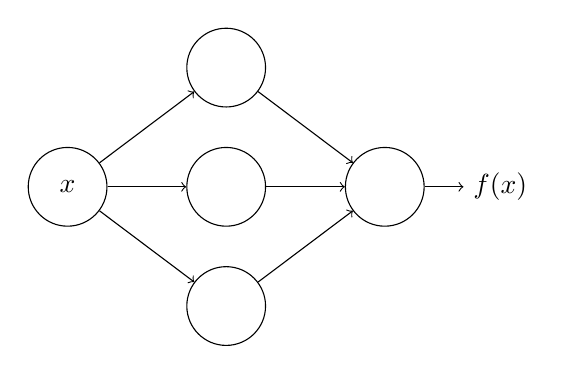
\begin{tikzpicture}[
    neuron/.style={circle,draw,inner sep=0pt,minimum size=10mm}
    ]
    
    \node (m1) [neuron] {};
    \node (m0) [neuron,below=.5 of m1] {};
    \node (m2) [neuron,above=.5 of m1] {};
    \node (l0) [neuron,left=of m1] {$x$};
    \node (r0) [neuron,right=of m1] {};
    
    \foreach \x in {0,1,2}
      \draw[->] (l0) to (m\x);

    \foreach \x in {0,1,2}
      \draw[->] (m\x) to (r0);
      
    \draw[->] (r0) -- ++(1,0) node [right] {$f(x)$};

  \end{tikzpicture} 
\end{document}
